\documentclass[12pt, a4paper]{article}
\usepackage[T2A]{fontenc}
\usepackage[utf8]{inputenc}
\usepackage[russian]{babel}
\usepackage{graphicx}
\usepackage{amsfonts}
\usepackage{indentfirst}
\usepackage{amsmath}
\usepackage{amsthm}
\usepackage{nicematrix}
\usepackage{hyperref}
\hypersetup{
    colorlinks=true,
    linkcolor=black,
    filecolor=magenta,      
    urlcolor=cyan,
    pdftitle={Lab4},
    pdfpagemode=FullScreen,
}
\usepackage{soulutf8}
\usepackage[left=1cm,right=1cm,
    top=2cm,bottom=2cm]{geometry}
\usepackage{titleps}
    \newpagestyle{main}{
        \setheadrule{0.4pt}
        \sethead{something}{\thepage}{}
}
\usepackage{listings}
\usepackage{color}

\definecolor{dkgreen}{rgb}{0,0.6,0}
\definecolor{gray}{rgb}{0.5,0.5,0.5}
\definecolor{mauve}{rgb}{0.58,0,0.82}

\lstset{frame=tb,
  language=Python,
  aboveskip=3mm,
  belowskip=3mm,
  showstringspaces=false,
  columns=flexible,
  basicstyle={\small\ttfamily},
  numbers=none,
  numberstyle=\tiny\color{gray},
  keywordstyle=\color{blue},
  commentstyle=\color{dkgreen},
  stringstyle=\color{mauve},
  breaklines=true,
  breakatwhitespace=true,
  tabsize=3
}
%\pagestyle{main}
\theoremstyle{plain}
\newtheorem{theorem}{Теорема}[section]
\newtheorem{corollary}{Следствие}[theorem]
\newtheorem*{example}{\textit{Пример}}
\newtheorem*{definition}{Определение}

\begin{document}
\begin{titlepage}
    \newpage
    \begin{center}
        \begin{tabular}{cc}
            \parbox{12cm}{\centering \textbf{НИУ ИТМО}} \\
            \\
            \hline
            \hline
        \end{tabular}
    \end{center}

    \begin{center}
        \caps{\textbf{Факультет систем управления и робототехники}}\\
    \end{center}

    \vspace{1cm}

    \begin{center}
        \textsc{Лабораторная работа №5 \\ по дисциплине <<Частотные методы>>}
    \end{center}

    \vspace{8em}

    \noindent Выполнил:  \hfill Гридусов Д.Д

    \vspace{20pt}
    \noindent Преподаватель: \hfill Перегудин А.А \\
    \\
    \vfill
    \begin{center}
        Санкт-Петербург \\2024 г.
    \end{center}

\end{titlepage}

\tableofcontents
\newpage

\section{Непрерывное и дискретное Фурье преобразование}
\subsection{Истиный образ Фурье}
\[
    \Pi(t) =  \begin{cases}
        1, |t| \leq \frac{1}{2}, \\
        0, |t| > \frac{1}{2}
    \end{cases}
\]
\begin{center}
    $\hat{\Pi}(\nu) = \int\limits_{-\infty}^{\infty}\Pi(t)e^{-2i\pi \nu t}dt
        = \int\limits_{-0.5}^{0.5}e^{-2i\pi \nu t}dt
        = -\frac{1}{2i\pi \nu}e^{-2i\pi \nu t}|_{-0.5}^{0.5}
        = -\frac{1}{2i\pi\nu}(e^{-i\pi\nu} - e^{i\pi\nu})
        = \frac{e^{i\pi\nu} - e^{-i\pi\nu}}{2i} \frac{1}{\pi \nu}
        = \frac{\sin\pi\nu}{\pi\nu}$
\end{center}
\begin{center}
    $\hat{\Pi}(\nu) = sinc(\nu)$
\end{center}

\noindent Построим графики функции и образа Фурье:
\begin{figure}[!htb]
    \centering 
    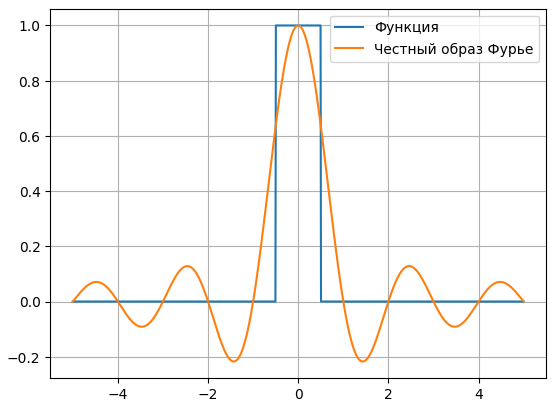
\includegraphics[scale=0.7]{../img/1}
    \caption{Аналитически найденный образ}
\end{figure}
 
\subsection{Образ через численное интегрирование}
\noindent Посчитаем тоже честный образ, но через аппроксимацию - используем функцию numpy.trapz
\\
\noindent \textbf{Листинг 1.1} Фурье-образ численным интегрированием
\begin{lstlisting}
def sq_wave(t):
    if (np.abs(t) <= 0.5):
        return 1
    return 0


def sq_wave_fourier_image(t):
    return np.sin(np.pi * t)/(np.pi * t)

# apply fourier transofrm using numerical integration
def trapz_ft(function, time, dt):
    def integrand(nu):
        integral = lambda t: function(t) * np.exp(-2j * np.pi * nu * t)
        temp = [integral(i) for i in time]
        return np.trapz(temp, time)
    return lambda t: integrand(t)

#apply inverse fourier transform via numerical integration
def trapz_inverse_ft(ft_function, time, dt):
    def integrand(t):
        integral = lambda nu: ft_function(nu) * np.exp(2j * np.pi * nu * t)
        temp = [integral(i) for i in time]
        return np.trapz(temp, time)
    return lambda t: integrand(t)
\end{lstlisting}

\noindent Посмотрим на результаты: 

\begin{figure}[!htb]
    \minipage{0.5\textwidth}
    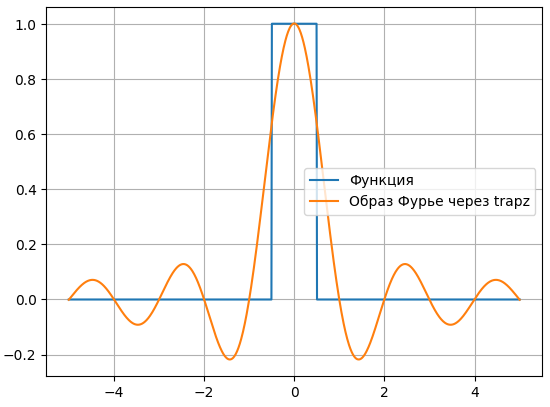
\includegraphics[width=\linewidth]{../img/2}
    \caption{Образ через численный подсчет}
    \endminipage\hfill
    \minipage{0.5\textwidth}
    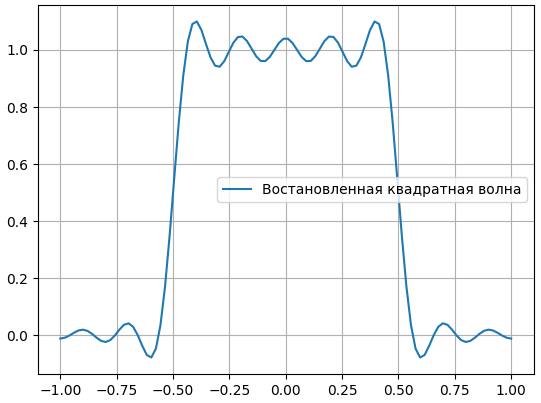
\includegraphics[width=\linewidth]{../img/3}   
    \caption{Обратное Фурье преобразование}
    \endminipage\hfill
\end{figure}
\noindent Образ Фурье был найден очень и очень точно, а с обратным возникли проблемы: во-первых, оно рассчитывалось минуты четыре, а во-вторых есть заметные отличия от исходной волны. Почему так произошло - будем разбираться позже, в отдельном пункте.
\newpage
\subsection{FFT}
\noindent Воспользуемся встроенной в nupmy быстрым преобразованием Фурье (FFT) и выведем результат: 
\begin{figure}[!htb]
    \minipage{0.5\textwidth}
    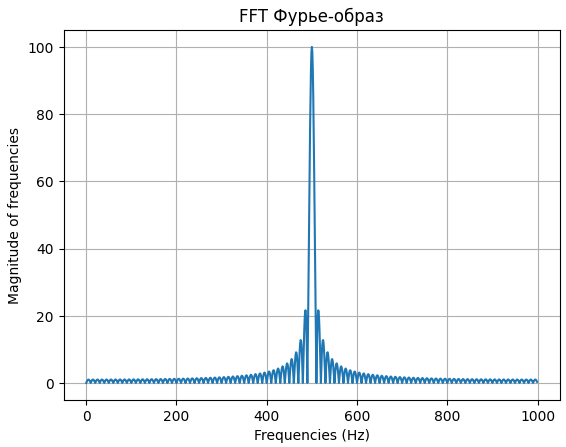
\includegraphics[width=\linewidth]{../img/4}
    \caption{Образ через DFT}
    \endminipage\hfill
    \minipage{0.5\textwidth}
    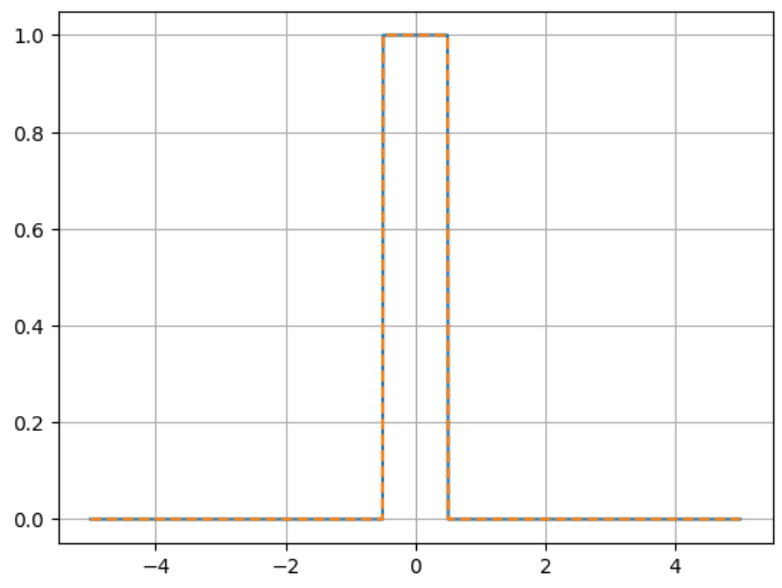
\includegraphics[width=\linewidth]{../img/5}   
    \caption{Обратное Фурье преобразование IFFT}
    \endminipage\hfill
\end{figure}
\\
Видно, что получился точно не кардинальный синус.
Зато обратное преобразование Фурье сработало идеально
(пунктирный оранжевый сигнал - восстановленый, синий - исходный)

\subsection{Почему так?}

\noindent \textbf{Отличие образов:} аналитически найденный образ Фурье от квадратной волны - кардинальный синус. Кардинальный синус - это непрерывная функция. И используя численное интегрирование мы честно (с небольшой погрешностью) искали образ Фурье от непериодической функции непрерывного аргумента. В таком случае образом Фурье будет непрервная функци я - sinc, в данном случае. Используя дискретное преобразование Фурье (DFT) мы можем получить лишь функцию дискретного аргумента в качестве образа Фурье - то есть точно не кардинальный синус.
\\
\noindent \textbf{Отличие в обратном Фурье преобразовании}\\Видно, что DFT прекрасно справляется с задачей восстановления сигнала. Объясняется это видимо теоремой Найквиста-Шеннона-Котельникова. Что касается неудачи численного метода, я думаю, что причина его неточности в том, что обратное преобразование фурье должно выдавать непрерывную функцию, а квадратная волна имеет разрыв. Поэтому с помощью численного интегрирования мы можем лишь приблизить исходную квадратную волну, но не можем получить в её точности.   

\noindent \section{Непрерывный образ через DFT}

\section{Сэмплирование}
\subsection{Синусы}

\noindent \textbf{Листинг 2.1} Зададимся параметрами и построим сигналы 
\begin{lstlisting}
a1 = 2
a2  = 3
w1 = 0.3
w2 = .5
phi1 = pi/2
phi2= pi/4

y = lambda t: a1 * sin(w1 * t + phi1)  + a2 * sin(w2 * t + phi2)
dt = 0.0001
time = np.linspace(-100, 100, int(1/dt))
short_time = np.linspace(-5*pi, 5*pi, int(1/dt))
Y = [y(t) for t in short_time]
\end{lstlisting}
\noindent Построим непрерывную функцию на небольшом промежутке, добавив сэмплированные точки (70 штук).
\begin{figure}[!htb]
    \centering
    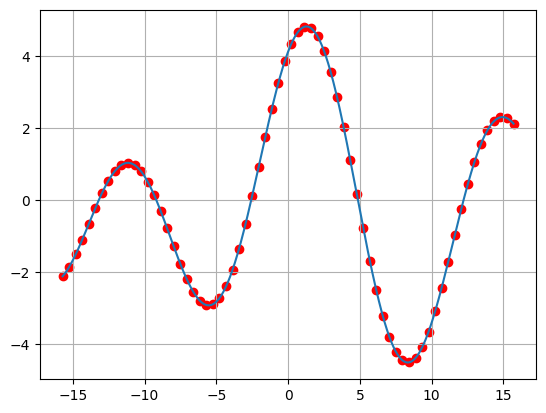
\includegraphics[scale=0.7]{../img/1_samples}
    \caption{Функция и ее дискретное разбиение, кол-во точек = 70}
\end{figure}

\noindent Применим дискретное преобразование Фурье 

\subsection{Кардинальные синусы}

\end{document}